\documentclass[nooutcomes]{ximera}

\input{../preamble}
\author{Kenneth Berglund}
\license{Creative Commons Attribution-ShareAlike 4.0 International License}
\acknowledgement{https://activecalculus.org/, stitz-zeager}

\title{Function Properties}

\begin{document}
\begin{abstract}
  
\end{abstract}
\maketitle


%\typeout{************************************************}
%\typeout{Motivating Questions}
%\typeout{************************************************}

\begin{motivatingQuestions}
\item What do we mean when we say a function is periodic?
\item What do we mean when we say a function is even or odd? How can we identify even and odd functions?
\end{motivatingQuestions}


%\typeout{************************************************}
%\typeout{Introduction}
%\typeout{************************************************}

When working with functions and looking at their graphs, we might notice some interesting patterns or behaviors. For example, a function like the sine function appears to repeat itself over and over again, and the quadratic function defined by $y = x^2$ appears to be symmetric about the $y$-axis. 

\begin{image}
\begin{tikzpicture}
    \begin{axis}[ymin=-2, ymax=2,
		   %xtick={-6.28318, -4.7123889, -3.14159, -1.5708, 1.5708, 3.14159, 4.7123889, 6.28318},
    xticklabels={
        $-\frac{3\pi}{2}$, $-\pi$, $\frac{\pi}{2}$, $0$,
        $\frac{\pi}{2}$, $\pi$, $\frac{3\pi}{2}$, $2\pi$
    }, title={$y = \sin(x)$}]
        \addplot[samples=200]{sin(pi/4*deg(x))};
    \end{axis}
\end{tikzpicture}

\begin{tikzpicture}
    \begin{axis}[title={$y = x^2$}]
        \addplot[smooth]{x^2} node{$y=x^2$};
    \end{axis}
\end{tikzpicture}
\end{image}

In this section, we'll discuss new vocabulary we can use to describe these behaviors as well as how to show analytically that a function has a certain behavior. 

We'll also discuss the important concept of inverse functions, which can provide a way to ``undo'' functions. 

%\typeout{************************************************}
%\typeout{Periodic functions}
%\typeout{************************************************}

\section{Periodic functions}

Certain naturally occurring phenomena eventually repeat themselves, especially when the phenomenon is somehow connected to a circle. For example, suppose that you are taking a ride on a ferris wheel and we consider your height, $h$, above the ground and how your height changes in tandem with the distance, $d$, that you have traveled around the wheel. We can see a full animation of this situation at \url{http://gvsu.edu/s/0Dt}. 

Because we have two quantities changing in tandem, it is natural to wonder if it is possible to represent one as a function of the other.

% Do I even want to go through an example like this or just use sine?

\begin{exploration}
In the context of the ferris wheel mentioned above, assume that the height, $h$, of the moving point (the cab in which you are riding), and the distance, $d$, that the point has traveled around the circumference of the ferris wheel are both measured in meters.

Further, assume that the circumference of the ferris wheel is 24 meters (it's a pretty short ferris wheel). In addition, suppose that after getting in your cab at the lowest point on the wheel, you traverse the full circle several times.

\begin{enumerate}
\item Recall that the circumference, $C$, of a circle is connected to the circle's radius, $r$, by the formula $C = 2\pi r$. What is the radius of the ferris wheel? How high is the highest point on the ferris wheel?

\item How high is the cab after it has traveled $\frac{1}{4}$ of the circumference of the circle?

\item How much distance along the circle has the cab traversed at the moment it first reaches a height of $\frac{12}{\pi} \approx 3.82$ meters?

\item Can $h$ be thought of as a function of $d$? Why or why not?

\item Can $d$ be thought of as a function of $h$? Why or why not?
\end{enumerate}
\end{exploration}



The natural phenomenon of a point moving around a circle leads to interesting relationships. Let's consider a point traversing a circle of circumference 24 and examine how the point's height, $h$, changes as the distance traversed, $d$, changes. Note particularly that each time the point traverses $\frac{1}{8}$ of the circumference of the circle, it travels a distance of $24 \cdot \frac{1}{8} = 3$ units, as seen below, where each noted point lies 3 additional units along the circle beyond the preceding one.


\begin{image}
\includegraphics[scale=.3]{traversing-first-example.pdf}
\end{image}


Note that we know the exact heights of certain points. Since the circle has circumference $C = 24$, we know that $24 = 2\pi r$ and therefore $r = \frac{12}{\pi} \approx 3.82$.  Hence, the point where $d = 6$ (located $1/4$ of the way along the circle) is at a height of $h = \frac{12}{\pi} \approx 3.82$.  Doubling this value, the point where $d = 12$ has height $h = \frac{24}{\pi} \approx 7.64$.  Other heights, such as those that correspond to $d = 3$ and $d = 15$ (identified on the figure by the green line segments) are not obvious from the circle's radius, but can be estimated from the grid in the figure above as $h \approx 1.1$ (for $d = 3$) and $h \approx 6.5$ (for $d = 15$).  Using all of these observations along with the symmetry of the circle, we can construct a table..

\begin{center}
\(
\begin{array}{ |c || c|  }
 \hline
 d & h\\
 \hline
 0&0\\
 3&1.1\\
 6&3.82\\
 9&6.5\\
 12&7.64\\
 15&6.5\\
 18&3.82\\
 21&1.1\\
 24&0\\
 \hline
\end{array}
\)
\end{center}

Moreover, if we now let the point continue traversing the circle, we observe that the $d$-values will increase accordingly, but the $h$-values will repeat according to the already-established pattern, resulting in the data in the table below.

\begin{center}
\(
\begin{array}{ |c || c|  }
 \hline
 d & h\\
 \hline
 24&0\\
 27&1.1\\
 30&3.82\\
 33&6.5\\
 36&7.64\\
 39&6.5\\
 42&3.82\\
 45&1.1\\
 48&0\\
 \hline
\end{array}
\)
\end{center}

It is apparent that each point on the circle corresponds to one and only one height, and thus we can view the height of a point as a function of the distance the point has traversed around the circle, say $h = f(d)$.  Using the data from the two tables and connecting the points in an intuitive way, we get the graph shown below

\begin{image}
\includegraphics{traversing-first-example-graph.pdf}
\end{image}

% How do I transition from that example to talking about periodicity

Notice that the graph above resembles the graph of the sine function. As it turns out, the sine function exhibits some of the same oscillatory behavior as $f$. This shared property turns out to be very important, especially when looking at functions that are related to circles. 

\begin{definition}
Let $f$ be a function whose domain and codomain % Have these been introduced?
are each the set of all real numbers. We say that $f$ is \index{function ! periodic}\index{periodic function}\dfn{periodic} provided that there exists a real number $k$ such that $f(x + k) = f(x)$ for every possible choice of $x$. The smallest value $p$ for which $f(x + p) = f(x)$ for every choice of $x$ is called the \index{period}\dfn{period} of $f$.

\end{definition}

For our ferris wheel example above, the period is the circumference of the circle that generates the curve. In the graph, we see how the curve has completed one full cycle of behavior every 24 units, regardless of where we start on the curve.

Later in the course, you will encounter and study many other examples of periodic functions.
 


%\typeout{************************************************}
%\typeout{Odd and even functions}
%\typeout{************************************************}

\section{Odd and even functions}

Consider the two functions, $g(x) = x$ and $h(x) = x^2$, whose graphs are shown below.
\begin{image}
\begin{tikzpicture}
    \begin{axis}[title={$g(x) = x$}]
        \addplot[smooth]{x} node{$g(x) = x$};
    \end{axis}
\end{tikzpicture}

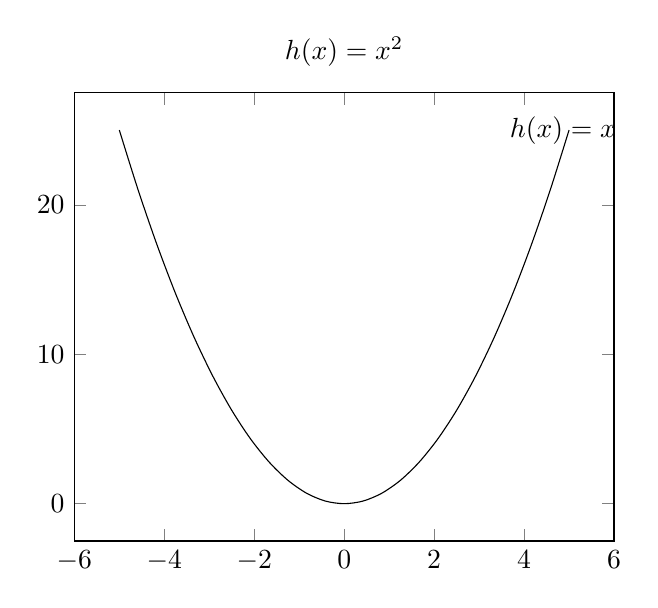
\begin{tikzpicture}
    \begin{axis}[title={$h(x) = x^2$}]
        \addplot[smooth]{x^2} node{$h(x)=x^2$};
    \end{axis}
\end{tikzpicture}
\end{image}

Note that the graph of $g$ seems to be symmetric about the origin, meaning that when we rotate the graph a half-turn, we get the same graph. Also, the graph of $h$ seems to be symmetric about the $y$-axis, meaning that when we flip the graph across the $y$-axis, we get the same graph. 

Let's first consider the case of $g$. To actually prove the symmetry about the origin analytically, we assume $(x,y)$ is a generic point on the graph of $g$. That is, we assume  $y = x$.  The point symmetric to $(x,y)$ about the origin is $(-x,-y)$.  To show the graph is symmetric about the origin, we need to show that $(-x,-y)$ is on the graph whenever $(x,y)$ is.  In other words, we need to show $(-x,-y)$ satisfies the equation $y = x$ whenever $(x,y)$ does.  Substituting $(-x, -y)$ into the equation gives
\begin{align*}
-y &\stackrel{?}{=} -x \\
y &\stackrel{\checkmark}{=} x.
\end{align*}

Since we are assuming the original equation $y = x$ is true, we have shown that $(-x, -y)$ satisfies the equation (since it leads to a true result) and hence, is on the graph of $g$. This shows that $g$ is symmetric about the origin.



\begin{exploration}
Consider the function $h$ defined by $h(x) = x^2$. We'll try to prove that $h$ is symmetric about the $y$-axis. 
\begin{enumerate}[label=\alph*.]
\item Assume $(x, y)$ is a generic point on the graph of $h$, so $y = x^2$. What point is symmetric to $(x, y)$ about the $y$-axis?
\item Show your answer to part a is on the graph of $h$ whenever $(x, y)$ is. Conclude that $h$ is symmetric about the $y$-axis. 
\end{enumerate}
\end{exploration}

Notice that to test an equation's graph for symmetry about the origin, we replaced $x$ and $y$ with $-x$ and $-y$, respectively.  Doing this substitution in the equation $y = f(x)$ results in $-y = f(-x)$.  Solving the latter equation for $y$ gives $y = -f(-x)$.  In order for this equation to be equivalent to the original equation $y=f(x)$ we need $-f(-x) = f(x)$, or, equivalently, $f(-x) = -f(x)$. In the exploration, you checked whether the graph of an equation was symmetric about the $y$-axis by replacing $x$ with $-x$ and checking to see if an equivalent equation results.  If we are graphing the equation $y=f(x)$, substituting $-x$ for $x$ results in the equation $y=f(-x)$.  In order for this equation to be equivalent to the original equation $y=f(x)$ we need $f(-x) = f(x)$. These results are summarized below.

The graph of a function $f$ is symmetric \index{symmetry ! testing a function graph for}

\begin{itemize}

\item  about the $y$-axis if and only if $f(-x) = f(x)$ for all $x$ in the domain of $f$.

\item  about the origin if and only if $f(-x) = -f(x)$ for all $x$ in the domain of $f$.

\end{itemize}

\begin{definition}
We call a function \index{function ! even}\index{even function}\dfn{even} if its graph is symmetric about the $y$-axis or \index{function ! odd}\index{odd function}\dfn{odd} if its graph is symmetric about the origin.  Apart from a very specialized family of functions which are both even and odd, functions fall into one of three distinct categories: even, odd, or neither even nor odd.  
\end{definition}

\begin{example}
Determine analytically if the following functions are even, odd, or neither even nor odd. 
\begin{enumerate}
\item $f(x) = \frac{5}{2 - x^2}$ 
\item $g(x) = \frac{5x}{2 - x^2}$ 
\item $h(x) = \frac{5x}{2 - x^3}$
\end{enumerate}
\end{example}


\begin{explanation}
The first step in all these problems is to replace $x$ with $-x$ and simplify.

\begin{enumerate}
\item Here, $f(x) = \frac{5}{2 - x^2}$. Replacing $x$ with $-x$, we find that

\begin{align*}
f(-x) & = \frac{5}{2 - (-x)^2}\\
f(-x) & = \frac{5}{2 - x^2},
\end{align*}

so $f(-x) = f(x)$. This shows that $f$ is \emph{even}. 

\item Here, $g(x) = \frac{5x}{2 - x^2}$. Replacing $x$ with $-x$, we find that

\begin{align*}
g(-x) & = \frac{5(-x)}{2 - (-x)^2}\\
g(-x) & = \frac{-5x}{2 - x^2}.
\end{align*}

It doesn't appear that $g(-x)$ is equal to $g(x)$. To prove this, we check with an $x$ value. After some trial and error, we see that $g(1) = 5$ whereas $g(-1) = -5$. This proves that $g$ is not even, but it doesn't rule out the possibility that $g$ is odd. (Why not?) To check if $g$ is odd, we compare $g(-x)$ with $-g(x)$:

\begin{align*}
-g(x) & = -\frac{5x}{2 - x^2} \\
-g(x) & = \frac{-5x}{2 - x^2} \\
-g(x) & = g(-x).
\end{align*}
Since $-g(x) = g(-x)$, $g$ is \emph{odd}.

\item Here, $h(x) = \frac{5x}{2 - x^3}$. Replacing $x$ with $-x$, we find that 

\begin{align*}
h(-x) & = \frac{5(-x)}{2 - (-x)^3} \\
h(-x) & = \frac{-5x}{2 + x^3}.
\end{align*}

Once again, $h(-x)$ doesn't appear to be equal to $h(x)$. We check with an $x$ value. For example, $h(1) = 5$, but $h(-1) = -\frac{5}{3}$. This proves that $h$ is not even and it also shows $h$ is not odd. (Why?)

\end{enumerate}
\end{explanation}

\begin{summary}\begin{itemize}
\item For a function \(f\) defined on the real numbers, we say $f$ is periodic if there exists some $k$ such that
\begin{equation*}
f(x + k) = f(x)
\end{equation*}
for all possible choices of $x$. The smallest value of $k$ for which $f(x + k) = f(x)$ for all possible choices of $x$ is called the period of $f$.
\item A function $f$ is called
\begin{itemize}
\item even if $f(-x) = f(x)$ for all possible choices of $x$. Even functions are symmetric about the $y$-axis. 
\item odd if $f(-x) = -f(x)$ for all possible choices of $x$. Odd functions are symmetric about the origin. 
\end{itemize}
\end{itemize}\end{summary}


\end{document}
